\chapter{Experimental Tasks}

Before the tasks were performed the PIN diode was set into the test set-up. Therefore it was aligned into the optical path of the laser. To align the diode the laser was driven at a constant laser current. The position of diode was adjusted to maximize the photocurrent. 


Beside the laser light the diode detected extraneous light as well. This leads to an offset of the measured photocurrent. With the laser switched off a photocurrent varying between 2.2 and 2.4~$\upmu$A could be measured.

\section{Task 1: Field characteristic of a PIN diode I}
\label{T1}
\begin{figure}%
\centering
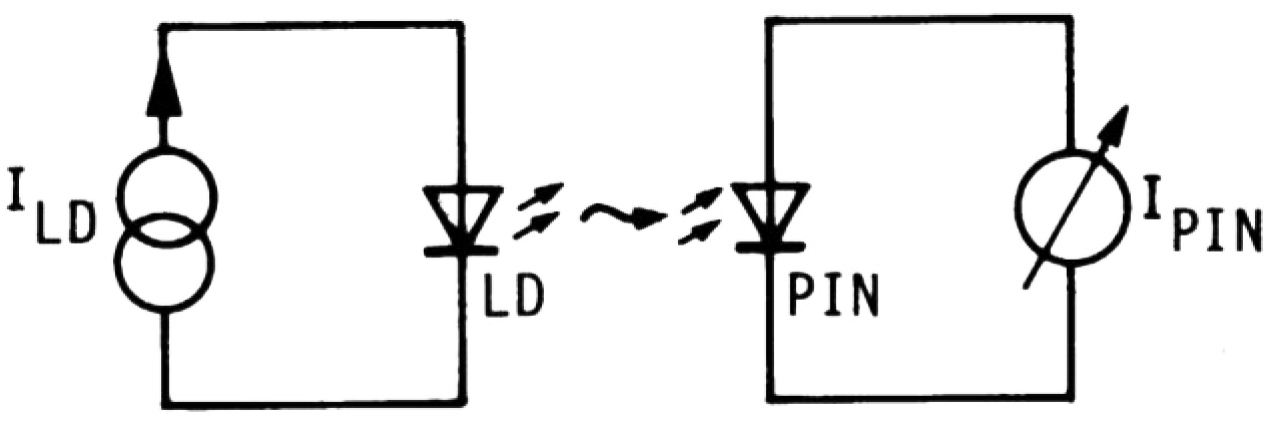
\includegraphics[width=.5\columnwidth]{Grafiken/T1_setup.jpg}%
\caption{Setup of task 1}%
\label{fig:T1_setup}%
\end{figure}
In this task the short-ci1rcuit current $I_{\mathrm{PIN}}$ of the PIN diode was measured for different laser currents. Figure \ref{fig:T1_setup}\footnote[3]{Source: OKT Experiment 2: Photodiode analysis task-sheet} shows the used setup. 

The laser current was swept from 0 to 60~mA. In the range from 0 to 10~mA a step size of the current change of 0.4~mA was used. From 10 to 20~mA the step size was 1~mA and from 20 to 60~mA a step size of 5~mA was used. 

\begin{figure}%
\centering
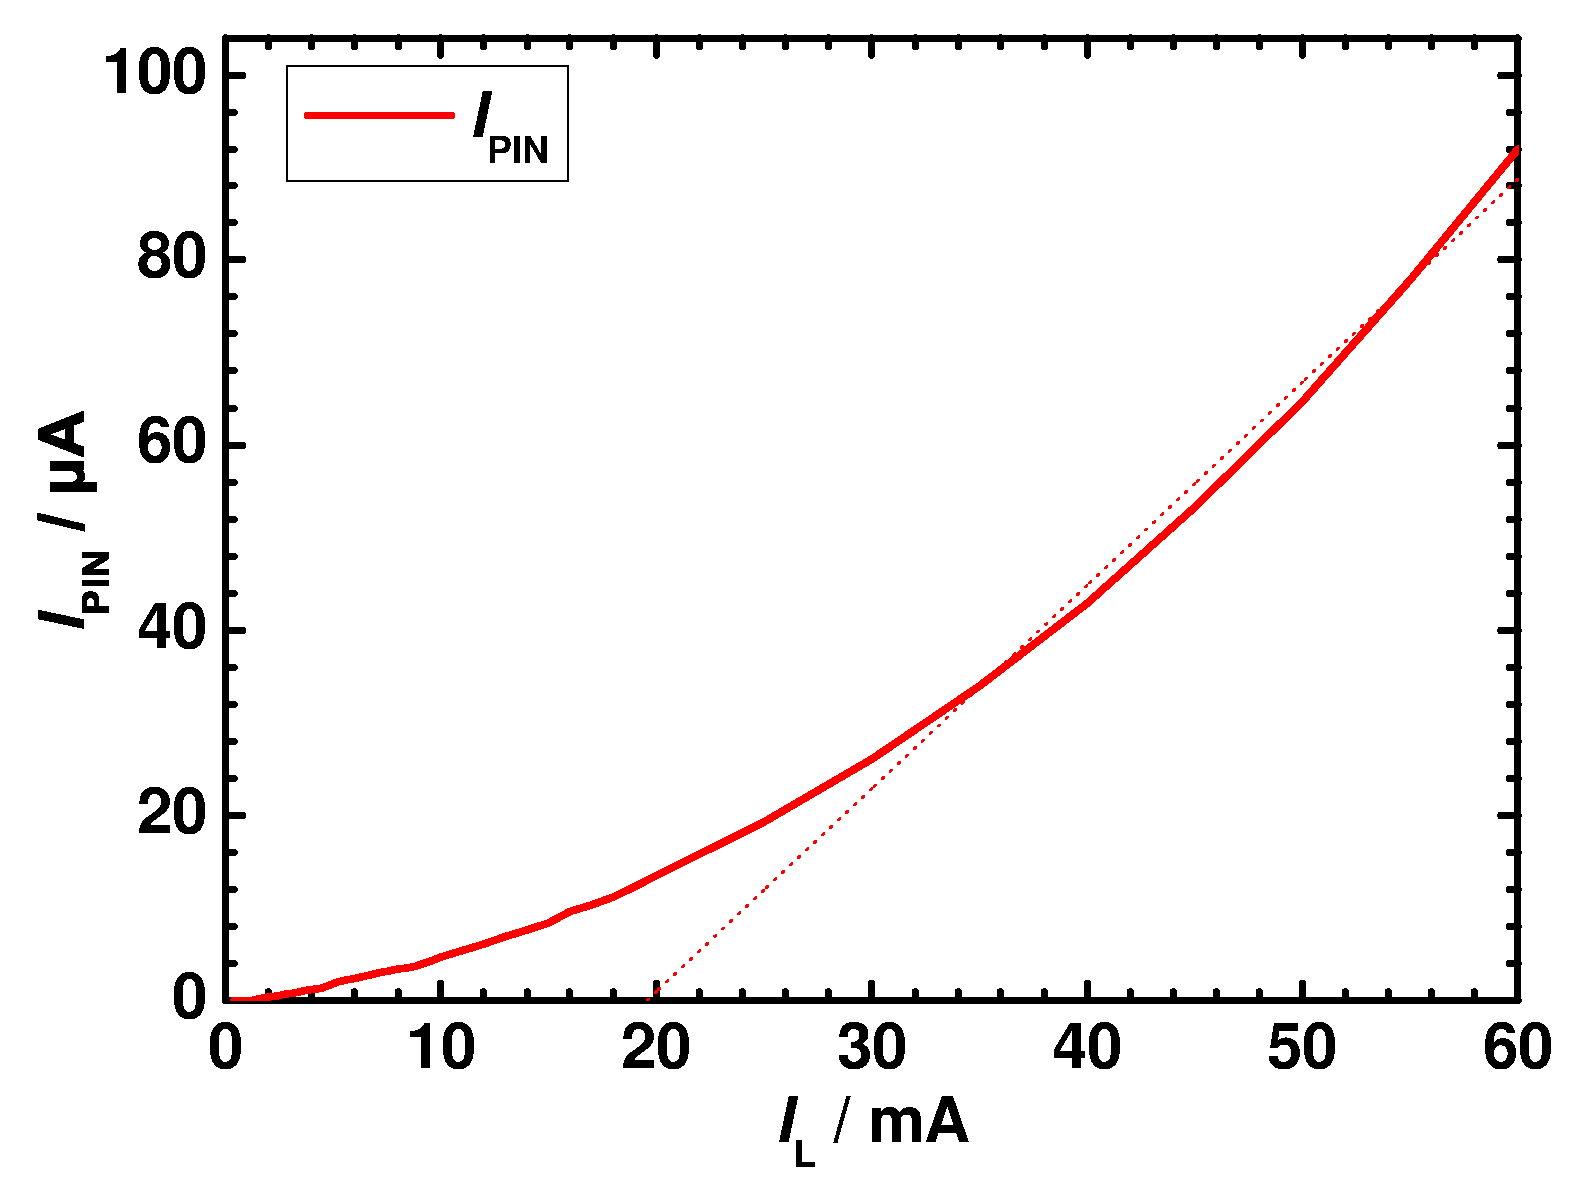
\includegraphics[width=.5\columnwidth]{Grafiken/T1_laser.pdf}%
\caption{Measured short-circuit currents.}%
\label{fig:T1_laser}%
\end{figure}

Figure \ref{fig:T1_laser} shows the measured short-circuit current $I_{\mathrm{PIN}}$ as a function of the laser current $I_{\mathrm{L}}$. Due to the fact that the measurement was not performed in a dark environment, the ambient light had impact on the measurements. For that reason the values of $I_{\mathrm{PIN}}$ are adjusted by 2.2~$\upmu$A. Thereby the value of $I_{\mathrm{PIN}}$ for the laser in off-state is 0~$\upmu$A.

To approximate the threshold a linear dependence of the number of photons emitted by the laser diode and the laser current was assumed \footnote[1]{Source: Optische Nachrichtentechnik; Grau,G; Freude, W; 3rd ed. Springer, 1991}. Since the power depends of the number of photons and the photocurrent is proportional to the laser power, the connection between $I_{\mathrm{PIN}}$ and $I_{\mathrm{L}}$ can be assumed as linear as well. The linear emission should start at the threshold current. Because of spontaneous emission in the laser diode the emission starts below this threshold.

To approximate the threshold a linear fitting of the curve was performed. Only values of $I_{\mathrm{L}} \geq 50$~mA were taken into account because the spontaneous emission is of no consequence there. This fit corresponds approximately to the tangent in the linear range. Figure \ref{fig:T1_laser} shows the linear fit as well. The intercept with $I_{\mathrm{PIN}} = 0~\upmu$A is at $I_{\mathrm{th}} \approx 28$mA. This can be assumed as the threshold of the laser diode.

For the next tasks four laser currents were selected. The corresponding photocurrents are equidistant. Table \ref{tab:T1_values} shows the selected currents. Since the photocurrent is proportional to the incoming radiant power, the corresponding powers at the four laser currents are equidistant as well.


\begin{table}%
\centering
\caption{Laser currents and corresponding primary photocurrents.}

\begin{tabular}{cc}

\toprule
$I_{\mathrm{L}}$ / mA	&	($I_{\mathrm{pr}}$ = -$I_{\mathrm{PIN}}$) / $\upmu$A\\

\midrule

19.5&15.0\\
31.4&30.0\\
40.0&45.0\\
47.1&60.0\\
\bottomrule 
\end{tabular}
\label{tab:T1_values}
\end{table}

\section{Task 2: Field characteristic of a PIN diode II}

In the second task first a bias is applied to the PIN-diode (cf. \ref{fig:T2_setup}). The voltage is varied from 0.1~V to 0.6~V and  $I_{\mathrm{PIN}}$ is recorded for the four $I_{\mathrm{pr}}$ determined in the first task (cf tabular \ref{tab:T1_values}). The voltage $U_{\mathrm{PIN0}} = U_{\mathrm{PIN}}(I_{\mathrm{PIN}}=0)$ is determined as well. For different laser currents and therefore different photo currents $U_{\mathrm{PIN0}}$ is quite different (cf. table \ref{tab:T2_voltage}). Figure \ref{fig:UPIN0} shows that $U_{\mathrm{PIN0}}$ is nearly exponentialy dependent on $I_{\mathrm{pr}}$. This can also be seen by using \eqref{eq:diode}. 
% \begin{equation}
%  \exp\frac{U_{\mathrm{PIN0}}}{U_{\mathrm{T}}} = \frac{I_{\mathrm{pr}}}{I_{\mathrm{sat}}} + 1
% \end{equation}


\begin{table}%
\centering
\caption{$U_{\mathrm{PIN}}(I_{\mathrm{PIN}}=0~\upmu$A) for different primary photocurrents.}

\begin{tabular}{cc}

\toprule
$I_{\mathrm{pr}} / \upmu$A & $U_{\mathrm{PIN}}(I_{\mathrm{PIN}} = 0~\upmu$A$) /$mV\\

\midrule
15.0 & 324\\
30.0 & 352\\
45.0 & 370\\
60.0 & 383\\

\bottomrule 
\end{tabular}
\label{tab:T2_voltage}
\end{table}



<<<<<<< HEAD
Next a reverse bias is applied to the PIN-diode. $U_{\mathrm{PIN}}$ is varied between 0 and -20~V and $I_{\mathrm{PIN}}$ is again recorded for the four $I_{\mathrm{pr}}$. Figure \ref{fig:linearity} shows the dependence of $I_{\mathrm{PIN}}$ on the photocurrent $I_{\mathrm{pr}}$ for a bias voltage of -4~V and -12~V respectively. One can see, that the dependency is linear. This dependency is the same for all measured reverse bias voltages. Thus $I_{\mathrm{PIN}}$ depends lineary on the photocurrent $I_{\mathrm{pr}}$ independent from the bias voltage as expected when looking at \eqref{eq:diode}.
=======
Figure \ref{fig:UPIN0} shows the dependency of $\exp(U_{\mathrm{PIN0}}/U_{\mathrm{T}})$ on $I_{\mathrm{pr}}$. \todo{evtl was die grafik bedeutet.}

Next a reverse bias is applied to the PIN-diode. $U_{\mathrm{PIN}}$ is varied between 0 and -20~V and $I_{\mathrm{PIN}}$ is again recorded for the four $I_{\mathrm{pr}}$. Figure \ref{fig:linearity} shows the dependence of $I_{\mathrm{PIN}}$ on the primary photocurrent $I_{\mathrm{pr}}$ for a bias voltage of -4~V and -12~V respectively. One can see, that the dependency is linear. This dependency is the same for all measured reverse bias voltages. Thus $I_{\mathrm{PIN}}$ depends lineary on the photocurrent $I_{\mathrm{pr}}$ independent from the bias voltage as expected when looking at \eqref{eq:diode}.
>>>>>>> 02c9a384062676bae5f4b57592caf0434d4d899c

Figure \ref{fig:PIN_kombiniert} shows the field characteristic of the PIN-diode for a forward bias as well as reverse bias voltage.
 


\begin{figure}%
\centering
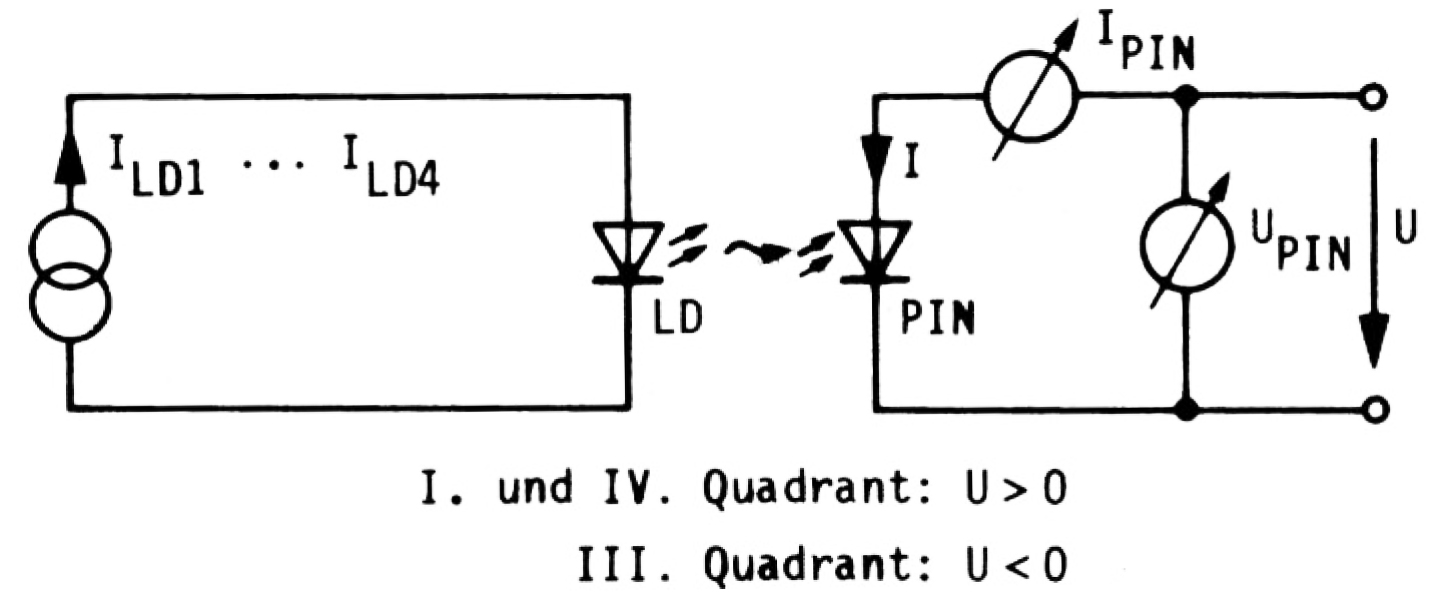
\includegraphics[width=.6\columnwidth]{Grafiken/T2_setup.jpg}%
\caption{Setup of task 2}%
\label{fig:T2_setup}%
\end{figure}

\begin{figure}%
\centering
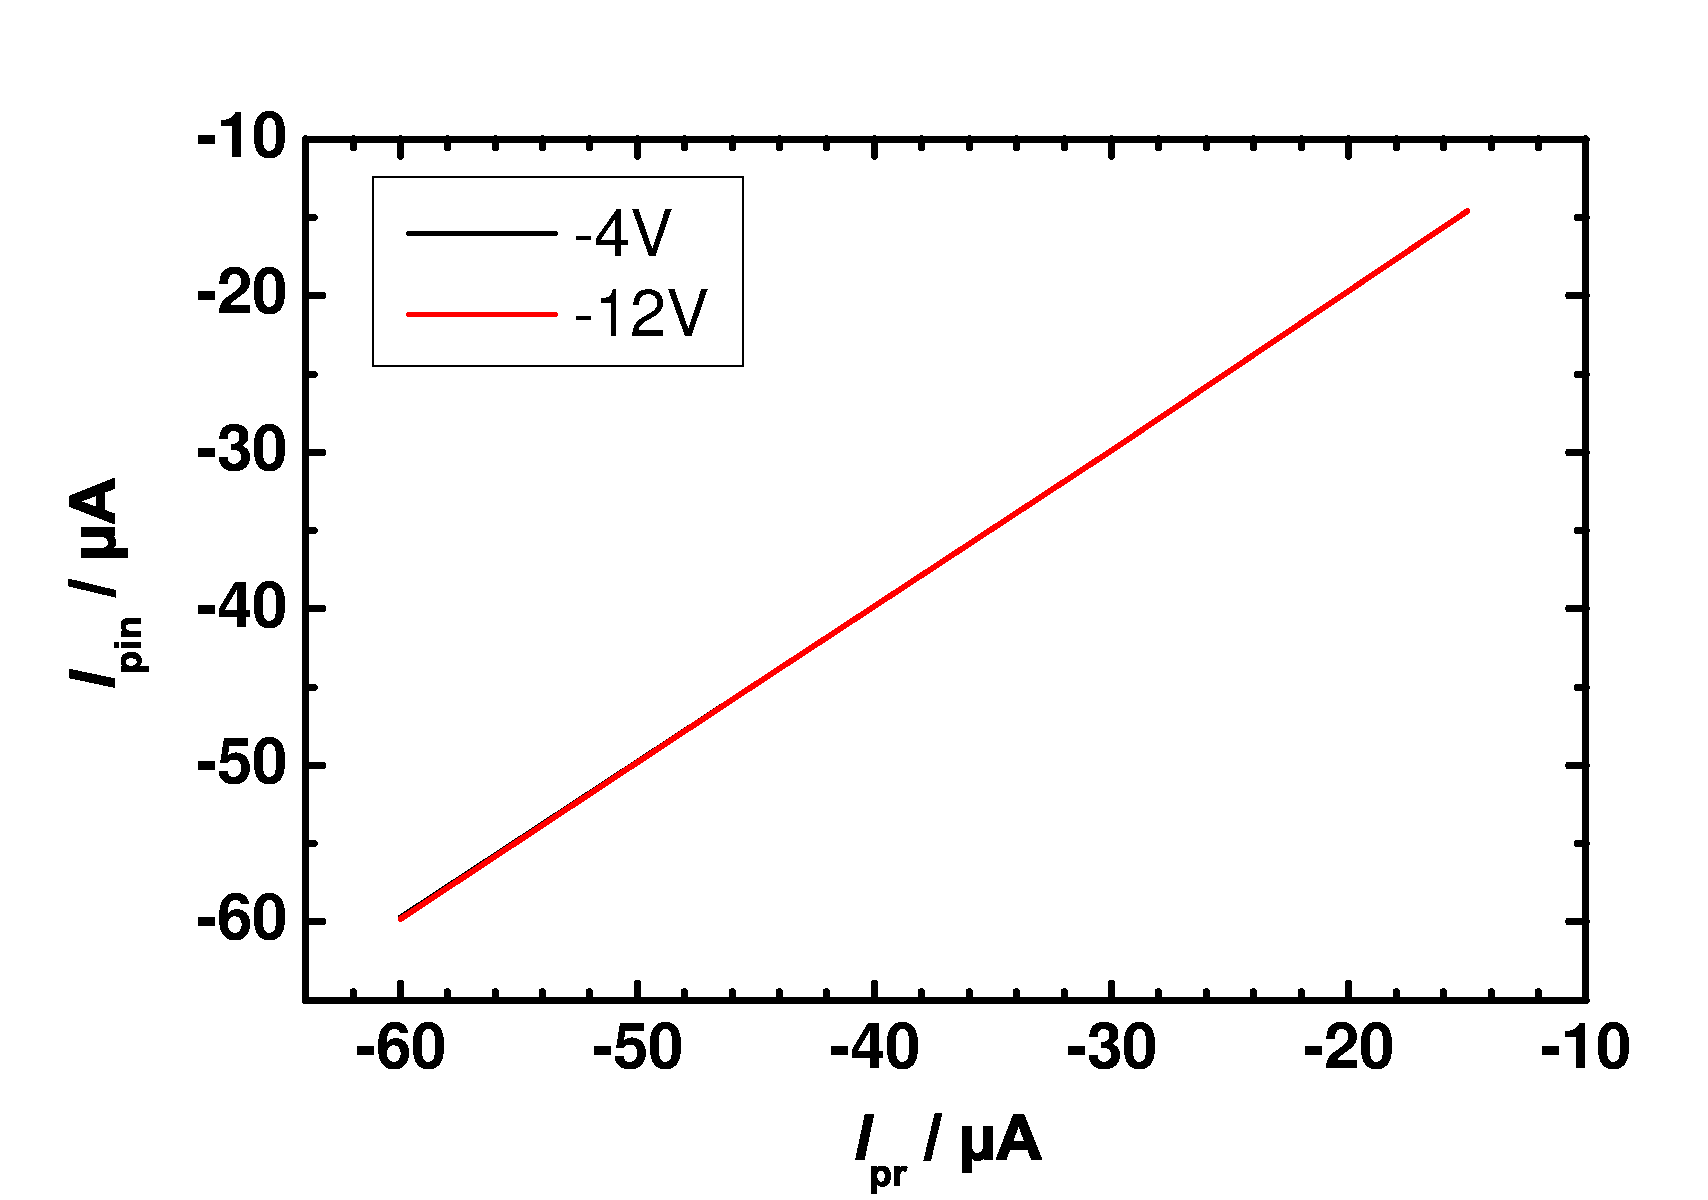
\includegraphics[width=.6\columnwidth]{Grafiken/linearity.pdf}%
\caption{Dependency of $I_{\mathrm{PIN}}$ on the primary photocurrent $I_{\mathrm{pr}}$}%
\label{fig:linearity}%
\end{figure}

\begin{figure}%
\centering
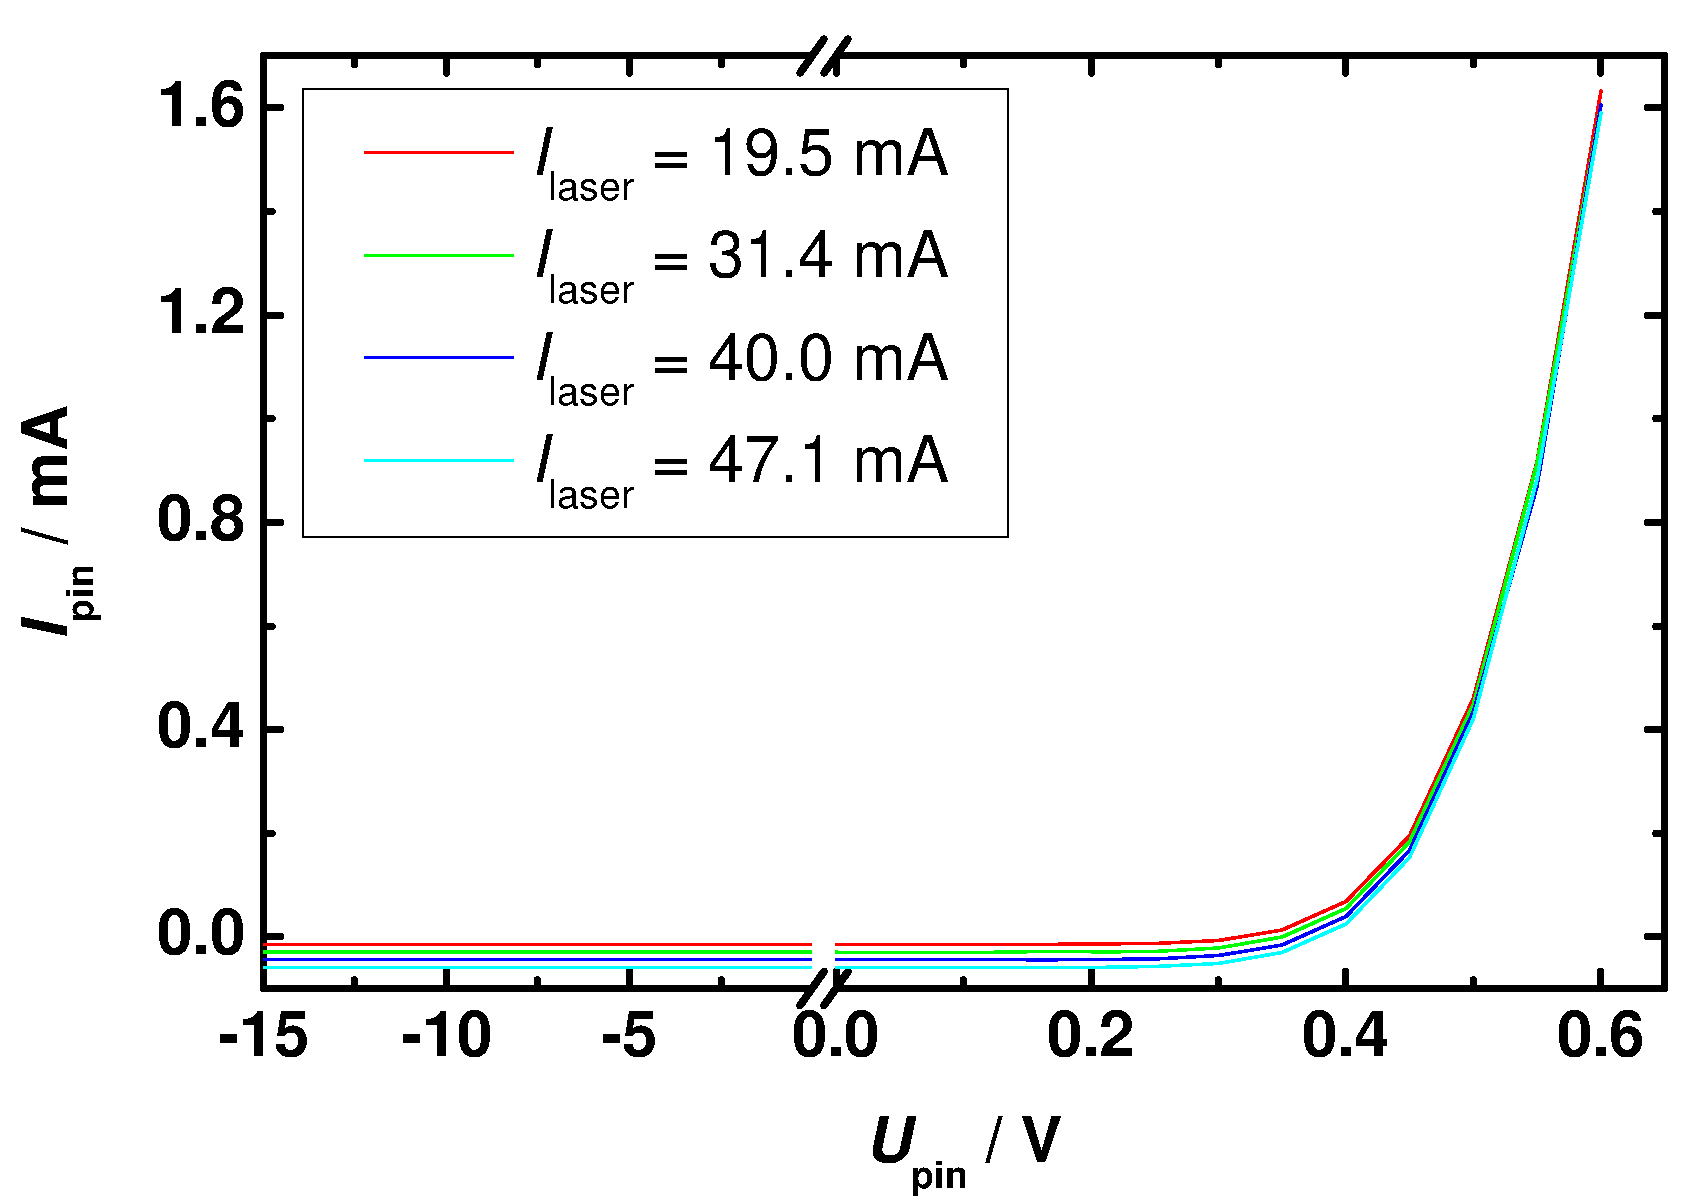
\includegraphics[width=.6\columnwidth]{Grafiken/PIN_kombiniert.pdf}%
\caption{Field characteristic of the PIN-diode}%
\label{fig:PIN_kombiniert}%
\end{figure}
\begin{figure}%
\centering
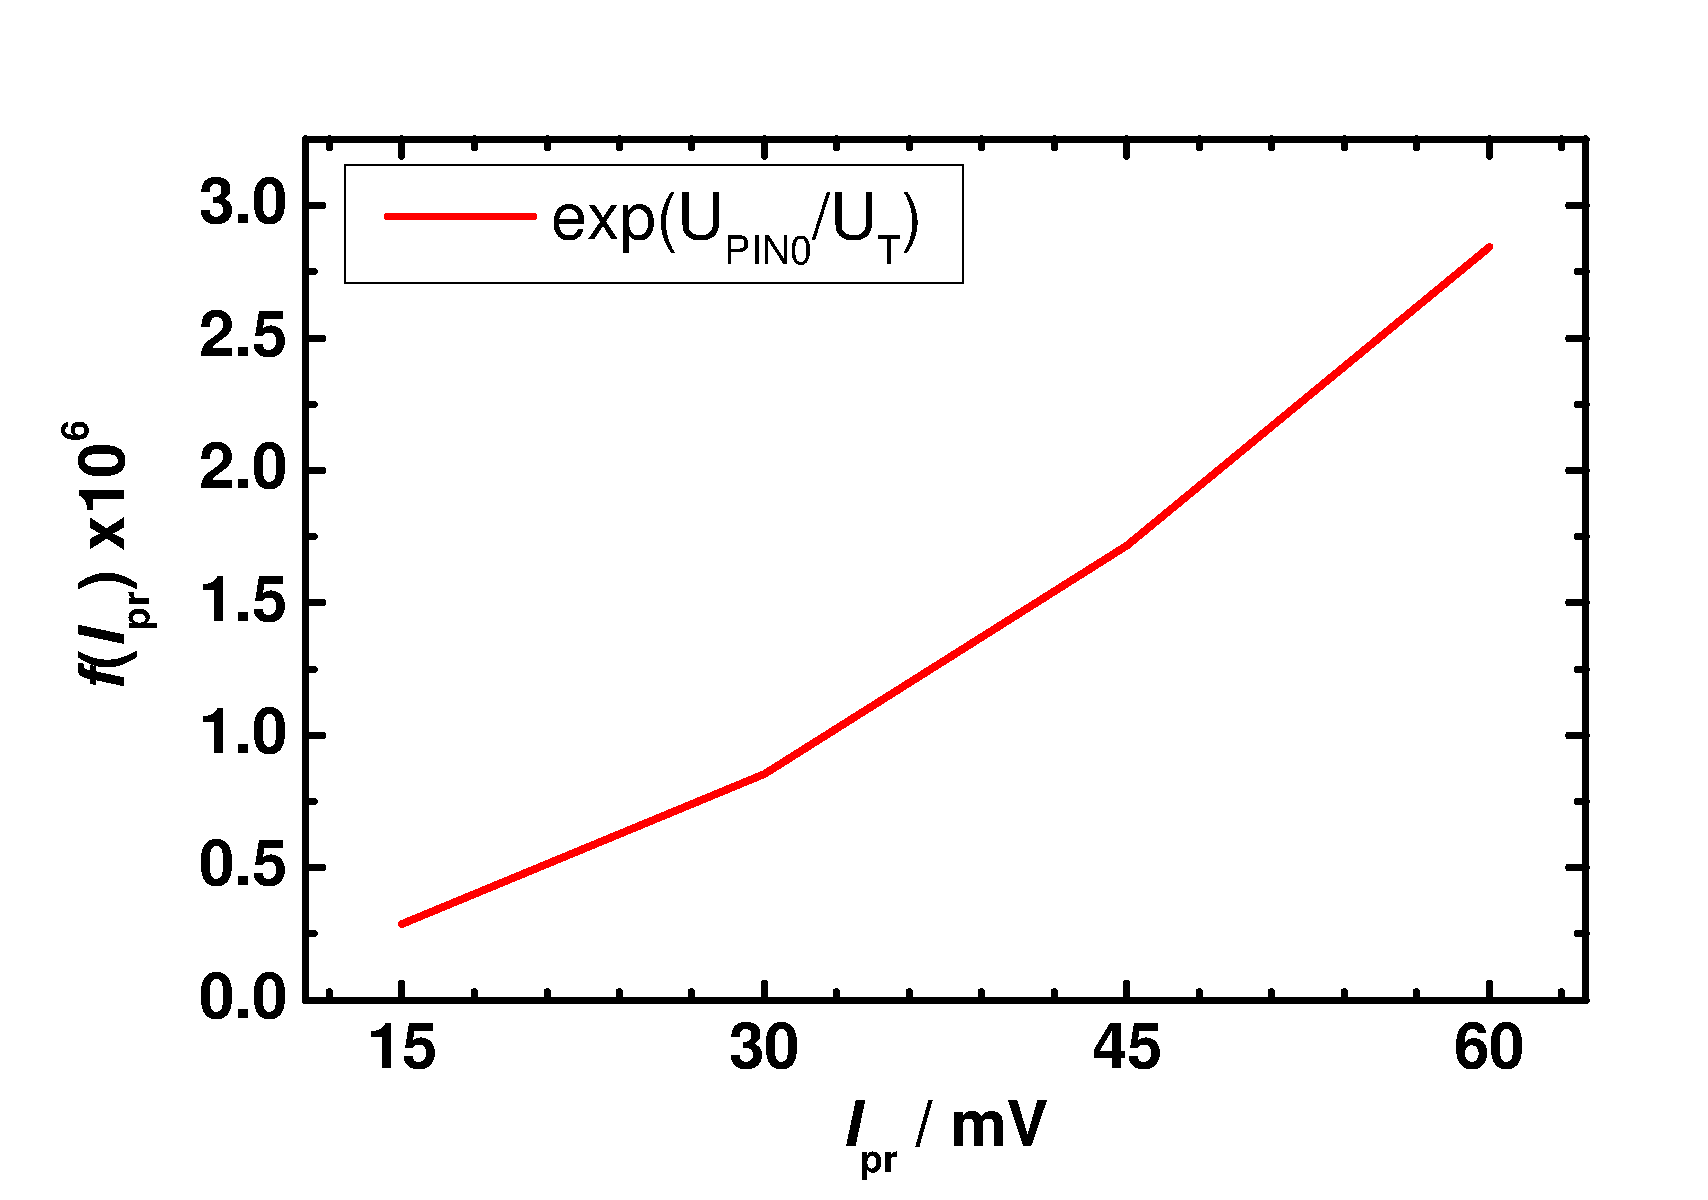
\includegraphics[width=.6\columnwidth]{Grafiken/UPIN0.pdf}%
\caption{Dependency of $\exp(U_{\mathrm{PIN0}}/U_{\mathrm{T}})$ on $I_{\mathrm{pr}}$}%
\label{fig:UPIN0}%
\end{figure}
\section{Task 3: Field characteristic of an APD}

For this task a APD was integrated into the setup. The diode was aligned to maximize the output current $I_{\mathrm{APD}}$.
Figure \ref{fig:T3_setup}\footnote[3]{Source: OKT Experiment 2: Photodiode analysis task-sheet} shows the setup.

To measure the caracteristic of the laser diode a reverse voltage ov $U = -10$~V was applied to the APD and the series resistance $R_{\mathrm{V}}$. ``The voltage corresponds to an avalanche multiplication factor $M_0 \approx 1$''\footnote[3]{Source: OKT Experiment 2: Photodiode analysis task-sheet}.

\begin{figure}%
\centering
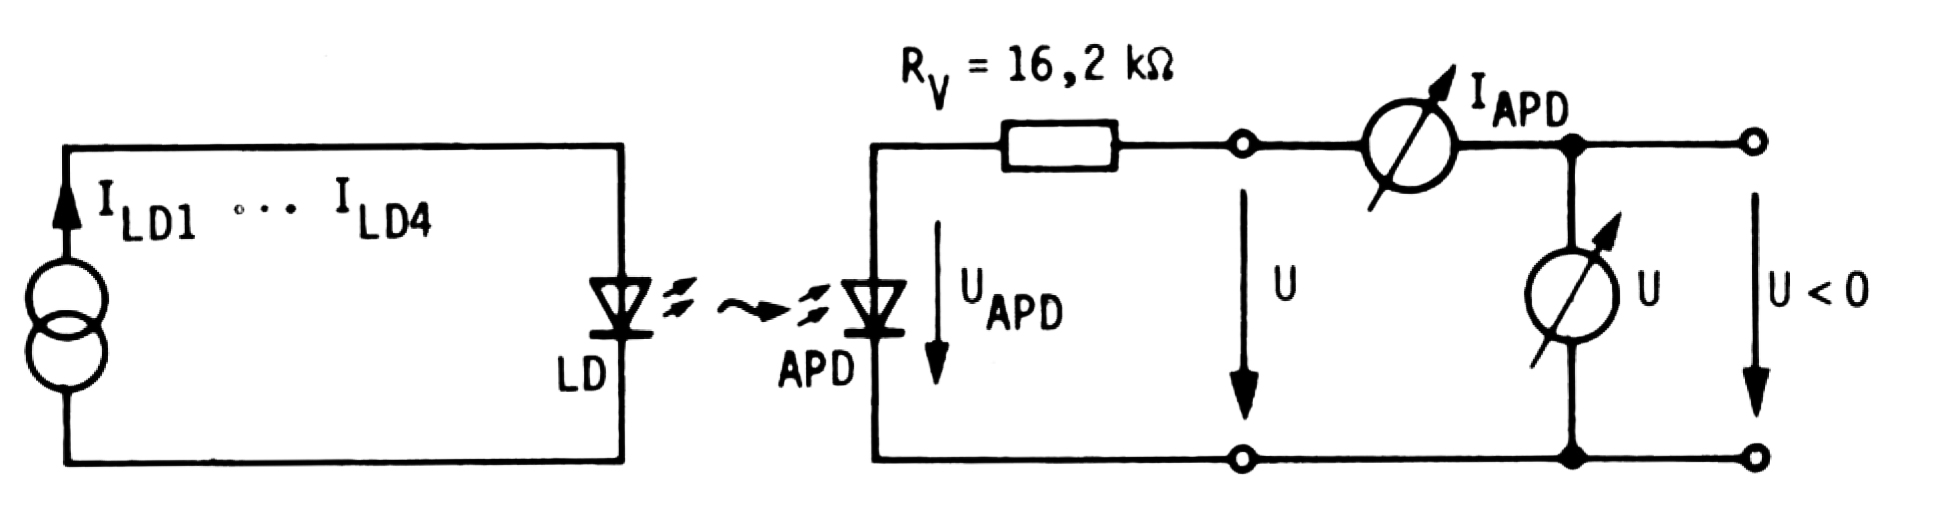
\includegraphics[width=.85\columnwidth]{Grafiken/T3_setup.jpg}%
\caption{Setup of task 3}%
\label{fig:T3_setup}%
\end{figure}


\begin{figure}%
\centering
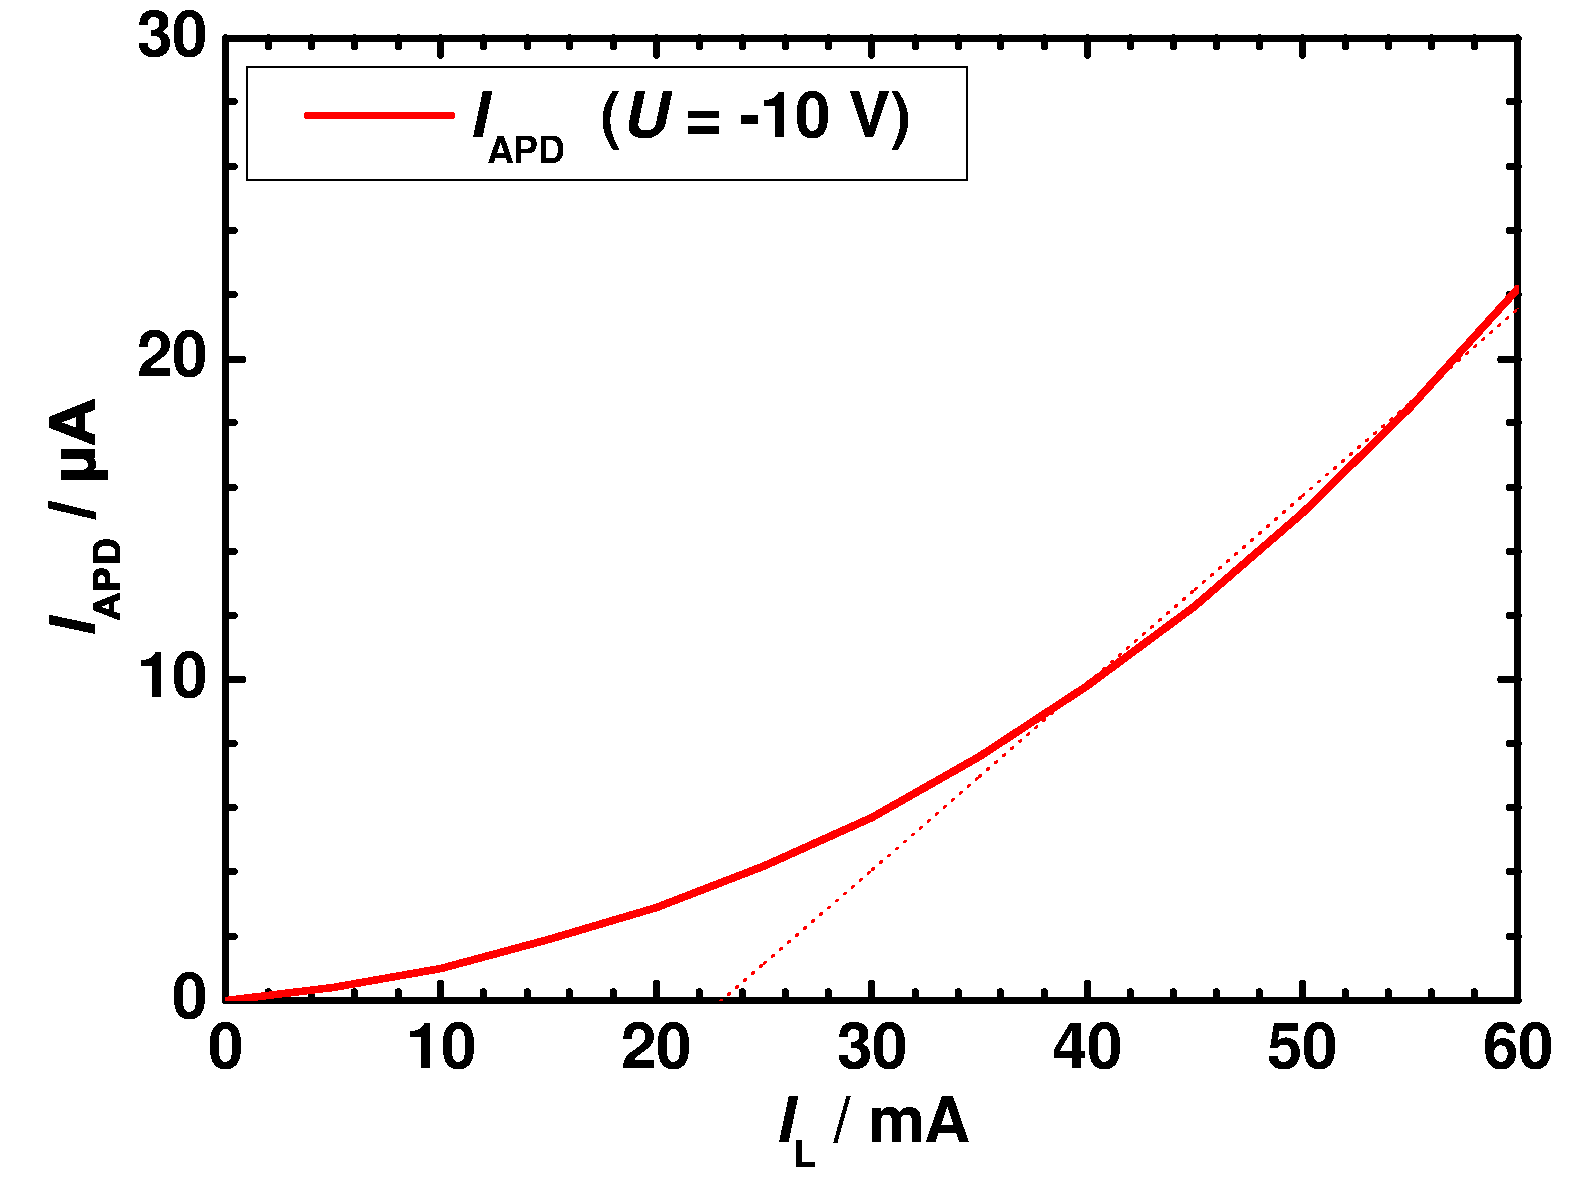
\includegraphics[width=.5\columnwidth]{Grafiken/T3_laser.pdf}%
\caption{Dependency of the primary photocurrent of the APD on the laser current.}%
\label{fig:T3_laser}%
\end{figure}


A laser current range from 0~mA~$\leq I_{\mathrm{L}} \leq 60$~mA was swept in 5~mA steps. There was no offset of $I_{\mathrm{APD}}$ when the laser was switched off. 

Figure \ref{fig:T3_laser} shows the measured photocurrent $I_{\mathrm{APD}}$ as a function of the laser current $I_{\mathrm{L}}$. 

The approximation of the threshold was performed as in \ref{T1} described.
With this linear approximation for $I_{\mathrm{L}} \geq 50$~mA a threshold of $I_{\mathrm{th}} \approx 30$~mA can be read off.

This is near the value determined by using the PIN diode but not the same. The used method is sufficient to approximate the threshold current but to inaccurate for an exact determination.   



Similar to \ref{T1} four laser currents were selected. The corresponding photocurrents are equidistant (cf. tab. \ref{tab:T3_values}).

\begin{table}%
\centering
\caption{Laser currents and corresponding primary photocurrents at a reverse voltage of $U = -10$~V.}


\begin{tabular}{cc}

\toprule
$I_{\mathrm{L}}$ / mA	&	$I_{\mathrm{pr}}$ / $\upmu$A\\

\midrule
27.6 & -5\\
40.5 & -10\\
40.7 & -15\\
57.1 & -20\\

\bottomrule 
\end{tabular}
\label{tab:T3_values}
\end{table}

For this four laser currents the dependency of $I_{\mathrm{APD}}$ on the voltage $U$ was measured. The voltage was varied between -10~V and -150~V in steps of 10~V. Between -150~V and -160~V in steps of 2~V. The voltage $U_{\mathrm{APD}}$ over the photo diode is given by 

\begin{equation}
U_{\mathrm{APD}} = U - R_{\mathrm{V}}\cdot I_{\mathrm{APD}}, \qquad  R_{\mathrm{V}} = 16.2 \mathrm{kV}
\label{eq:}
\end{equation}
for $U < 0$~V and $I_{\mathrm{APD}} < 0~\upmu$A.

\begin{figure}%
\centering
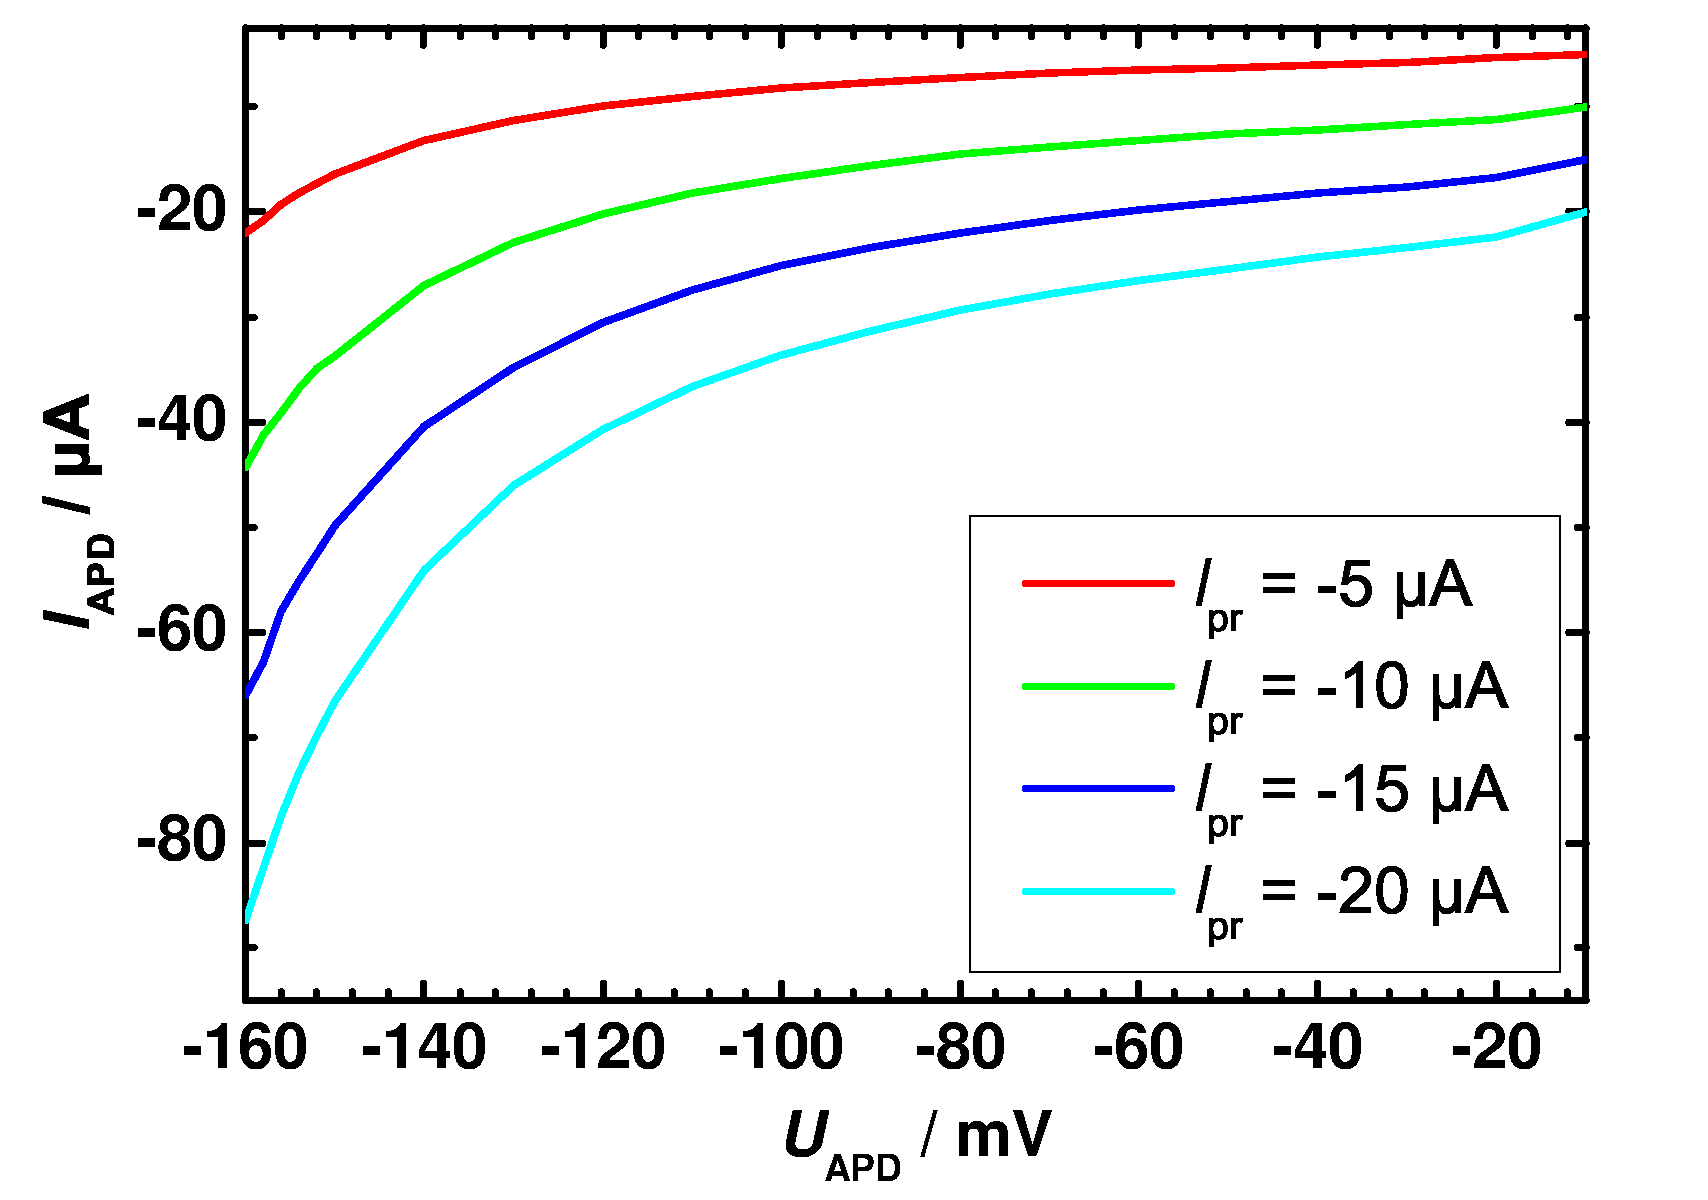
\includegraphics[width=.5\columnwidth]{Grafiken/T3_1.pdf}%
\caption{Relationship between  $I_{\mathrm{APD}}$,  $U_{\mathrm{APD}}$ and  $I_{\mathrm{pr}}$. }%
\label{fig:T3_1}%
\end{figure}

Figure \ref{fig:T3_1} shows the relationship between $I_{\mathrm{APD}}$,  $U_{\mathrm{APD}}$ and  $I_{\mathrm{pr}}$.
For $U_{\mathrm{APD}} < -120$~V the diode gets nonlinear. 

Figure \ref{fig:T3_2} shows the linear dependency of $I_{\mathrm{APD}}$ on $I_{\mathrm{pr}}$ for different voltages $U_{\mathrm{APD}}$ in the range of $-5~\upmu\mathrm{A} \geq I_{\mathrm{pr}} \geq - 20~\upmu\mathrm{A}$. With a higher voltage $U_{\mathrm{APD}}$ the slope gets steeper and the diode more sensitive.

\begin{figure}%
\centering
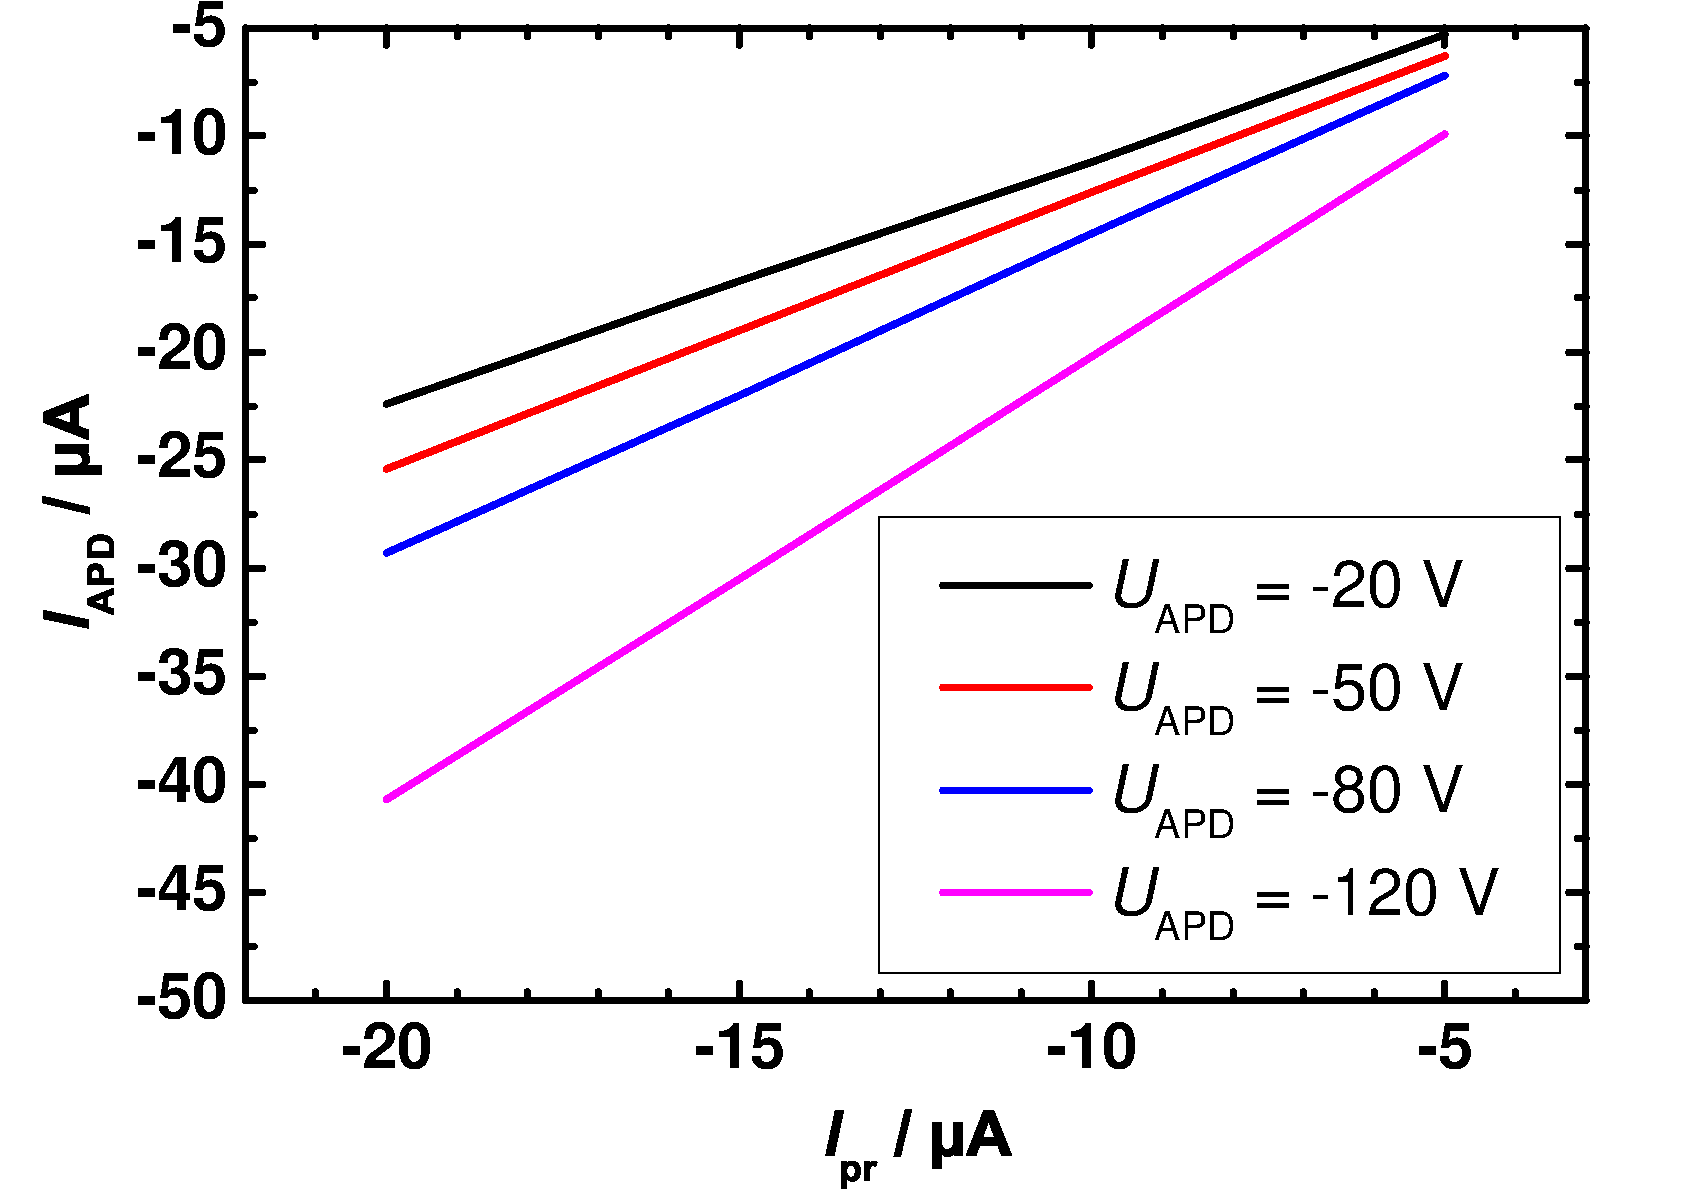
\includegraphics[width=.5\columnwidth]{Grafiken/T3_2.pdf}%
\caption{Linear dependency of $I_{\mathrm{APD}}$ on $I_{\mathrm{pr}}$ for different $U_{\mathrm{APD}}$.}%
\label{fig:T3_2}%
\end{figure}

The avalanche multiplication factor estimated by the formula

\begin{equation}
M_0(U_{\mathrm{APD}})=\frac{I_{\mathrm{APD}}(U_{\mathrm{APD}})}{I_{\mathrm{APD}}(U_{\mathrm{APD,min}}=-10\mathrm{~V})}.
\label{eq:M0}
\end{equation}

This function is plotted in figure \ref{fig:T3_3} for a photocurrent $I_{\mathrm{pr}}=-20~\upmu$A . To estimate the breakthrough voltage $U_{\mathrm{BR}}$ of the APD another formula\footnote[2]{Source: Optical Communication Systems - Part 2, Wolfgang Freude} for $M_0$ was was used:
\begin{equation}
M_{\mathrm{th}} = \frac{1}{1-(U/U_{\mathrm{BR}})^n},
\label{eq:Mth}
\end{equation}
where $n$ is an adaption parameter. 
This function was fitted to the values of $M_0$. The resulting function is

\begin{equation}
M_{\mathrm{th}} = \frac{1}{1-(\frac{U}{-190~\mathrm{V}})^{1.44}},\qquad U_{\mathrm{BR}}=-190~\mathrm{V}
\label{eq:M_fit}
\end{equation}
which is also plotted in figure \ref{fig:T3_3}.
With that the breakthrough voltage can be estimated as -190~V.

\begin{figure}%
\centering
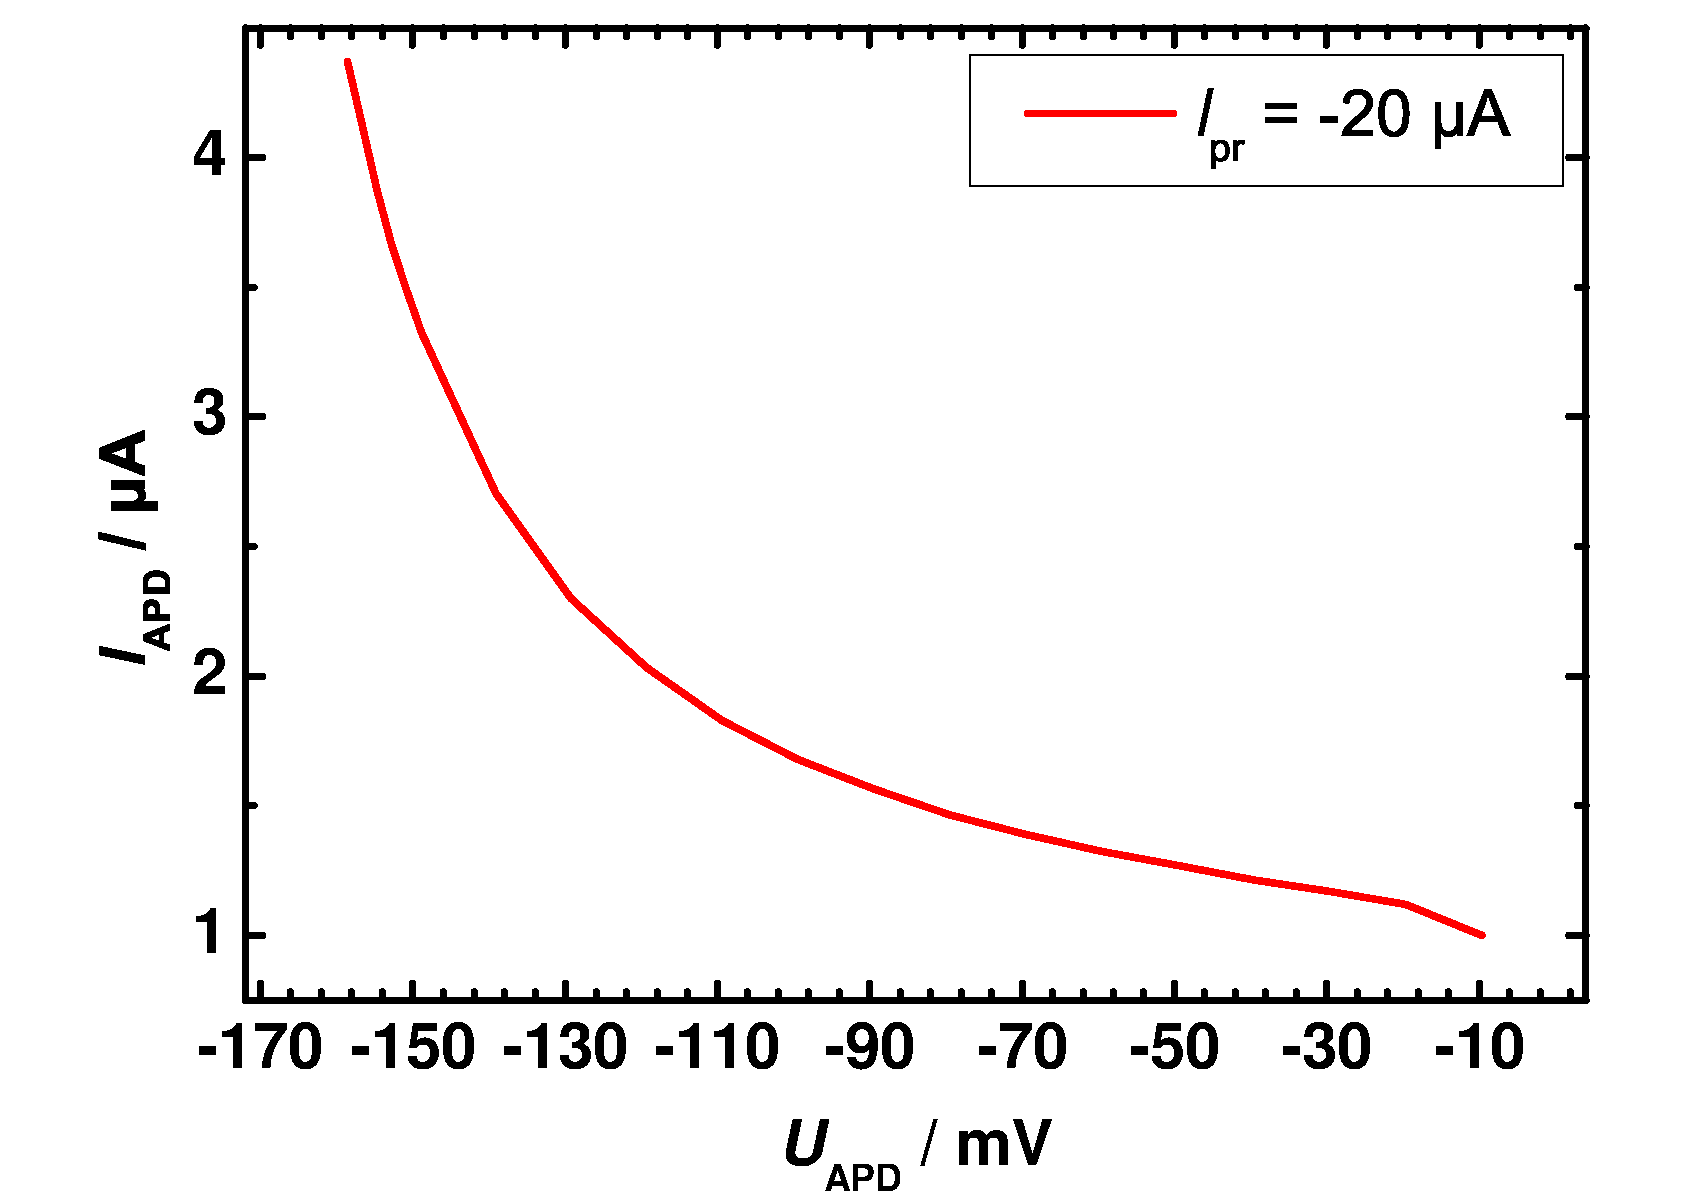
\includegraphics[width=.5\columnwidth]{Grafiken/T3_3.pdf}%
\caption{Calculated multiplication factor $M_0$ and theoretical multiplication factor $M_{\mathrm{th}}$ over $U_{\mathrm{APD}}$.}%
\label{fig:T3_3}%
\end{figure}